\section{Results}
\label{sec:results}

All comparisons follow the paired protocol of
Section~\ref{sec:experiments}: within each $(\mathrm{seed},\rho)$ cell, the
methods share partitions, sampled coordinates, and noisy sparse observations.
Method orderings in this section refer to the reported mean metrics across the
paired seeds.

\subsection{Cross-well low-data results}
\label{subsec:crosswell_results}

Table~\ref{tab:crosswell_clp_vs_ae} compares CLP-CSGM Ridge with AE
$[\boldsymbol{u},\boldsymbol{b}]$, the direct baseline with the lowest
unweighted mean RMSE across the grid. CLP-CSGM Ridge has lower mean RMSE in
seven of the nine cells; the exceptions are step $8$ with
$\rho\in\{0.05,0.10\}$. It has lower mean RMSE at every tested ratio for steps
$16$ and $32$. Across the three tested step sizes, the descriptive RMSE gap
shifts progressively in favor of CLP-CSGM as training support decreases.
At step $32$, the RMSE reductions relative to AE are approximately $32\%$ at
$\rho=0.10$ and $57\%$ at $\rho=0.20$.

Across the complete grid, the unweighted mean of the nine cell-level mean RMSE
values decreases from $0.03496$ for AE
$[\boldsymbol{u},\boldsymbol{b}]$ to $0.02862$ for CLP-CSGM Ridge, a reduction
of approximately $18.1\%$. The ordering still depends on the amount of
training data: the direct AE has lower mean RMSE in the two cells with the
largest training pool, step $8$ at $\rho=0.05$ and $\rho=0.10$.

\begin{table}[!htbp]
    \centering
    \caption{Cross-well $V_c$ comparison between CLP-CSGM Ridge and
    AE $[\boldsymbol{u},\boldsymbol{b}]$. Values are RMSE mean and standard
    deviation across seeds; a negative gap favors CLP-CSGM.}
    \label{tab:crosswell_clp_vs_ae}
    \small
    \adjustbox{max width=\linewidth}{
        \begin{tabular}{rrrrrrrr}
\toprule
step & n\_train\_approx & rho & clp\_csgm\_rmse\_mean & clp\_csgm\_rmse\_std & ae\_ub\_rmse\_mean & ae\_ub\_rmse\_std & gap\_vs\_ae\_pct \\
\midrule
8 & 104 & 0.05000 & 0.04483 & 0.00524 & 0.03567 & 0.00100 & 25.69014 \\
8 & 104 & 0.10000 & 0.03646 & 0.00194 & 0.03195 & 0.00208 & 14.10258 \\
8 & 104 & 0.20000 & 0.02267 & 0.00381 & 0.02600 & 0.00164 & -12.83374 \\
16 & 52 & 0.05000 & 0.03344 & 0.00151 & 0.03712 & 0.00098 & -9.91538 \\
16 & 52 & 0.10000 & 0.02689 & 0.00235 & 0.03420 & 0.00291 & -21.35910 \\
16 & 52 & 0.20000 & 0.01771 & 0.00138 & 0.03214 & 0.00742 & -44.89074 \\
32 & 27 & 0.05000 & 0.03217 & 0.00268 & 0.03901 & 0.00259 & -17.53826 \\
32 & 27 & 0.10000 & 0.02640 & 0.00342 & 0.03894 & 0.00228 & -32.21019 \\
32 & 27 & 0.20000 & 0.01705 & 0.00119 & 0.03959 & 0.00234 & -56.94200 \\
\bottomrule
\end{tabular}

    }
\end{table}

Table~\ref{tab:paired_delta_crosswell} reports the paired seed-wise difference
$\Delta\mathrm{RMSE}=\mathrm{RMSE}_{\mathrm{AE}}-\mathrm{RMSE}_{\mathrm{CLP}}$
with Student-$t$ half-widths ($\mathrm{df}=2$). At steps $16$ and $32$, where
training support is smallest, the
mean paired gap is positive at every $\rho$ and CLP-CSGM Ridge wins all three
seeds; at step $8$, where the development pool is largest, AE $[\boldsymbol{u},\boldsymbol{b}]$ wins the two
smallest $\rho$ cells, matching the mean-RMSE ordering in Table~\ref{tab:crosswell_clp_vs_ae}.
Several of these three-seed intervals include zero.
Appendix~\ref{app:crosswell_seed_panel} repeats the same pairwise comparison
on ten seeds: none of those intervals include zero. The CLP-CSGM advantage
remains in the few-window cells (steps $16$ and $32$); AE remains better at
step $8$ for $\rho=0.05$ and $\rho=0.10$.
Appendix~\ref{app:crosswell_explicit_mask} repeats the three-seed grid with
one extra direct AE that sees an explicit window mask. The mask does not
remove the CLP-CSGM advantage at steps $16$ and $32$. At step $8$ the masked
AE remains better at $\rho=0.05$ and $\rho=0.10$, and the mask does not
uniformly lower the direct AE error.

Appendix~\ref{app:crosswell_omega_placement} redraws the sparse coordinates
five times while the model seeds stay at $\{7,23,41\}$. The published cell
winner is unchanged in all nine cells. At steps $16$ and $32$, CLP-CSGM Ridge
has lower RMSE than AE $[\boldsymbol{u},\boldsymbol{b}]$ in every draw. At
step $8$, AE remains better at $\rho=0.05$ in every draw and at $\rho=0.10$
on the majority of draws; CLP-CSGM remains better at $\rho=0.20$ on the
majority of draws. The advantage where training support is smallest therefore
holds for every tested placement. Step $8$, where that support is largest,
remains the less stable regime.

Appendix~\ref{app:crosswell_simple_baselines} compares those same nine cells
with ordinary least squares and ridge regression from
$[\boldsymbol{u},\boldsymbol{b}]$, and with linear interpolation of the
sparse measurements along depth. The linear maps are scored at the published
noise standard deviation $0.01$. At that reference level, interpolation has
the lowest full-window RMSE in all nine cells and in all $27$ seed
comparisons. CLP-CSGM Ridge is lower than both direct linear maps at step
$16$, $\rho=0.20$, and at step $32$ for every $\rho$.

Figure~\ref{fig:crosswell_rmse_vs_noise} uses the same windows and changes
only the noise. Each panel is one step and each curve is one measurement
fraction, so the nine cells are not averaged together. At noise $0.01$,
interpolation has the lower error in all nine configurations. At noise
$0.05$, CLP-CSGM Ridge has the lower mean RMSE at steps $16$ and $32$ and
at step $8$ for $\rho=0.20$. At step $8$ for $\rho=0.05$ and $\rho=0.10$,
interpolation keeps the lower mean. At $0.10$ and $0.20$, CLP-CSGM Ridge
has the lower error in all nine configurations. The held-out $V_c$ curve
has standard deviation $0.035$, on the same scale as this noise. Relative
to that deviation, $0.05$ is about $1.43$ times larger, and $0.10$ and
$0.20$ are about $2.86$ and $5.71$ times larger. These noise levels were
used for sensitivity analysis and were not calibrated to field measurement
uncertainties. The decoder and the
dense-log map are fit once per step and seed. The penalty weight is then
selected on validation for each measurement fraction and each noise level,
so the curves are not a fixed-penalty reconstruction. The sensitivity sweep
uses a different, wider grid. The weight selected
at $0.01$ and at $0.05$ also belongs to the published grid. That membership
does not mean the two searches were the same. At noise $0.20$,
some cells select $100$, the largest candidate in the sweep grid. That
choice is the best value among the candidates that were tried, not an
optimum outside the grid. The points at
noise $0.01$ belong to this same refit: their ordering matches the
published grid, and the cell means can differ slightly from that grid.
The interpolation error grows with the noise because the interpolated curve
follows the measurements. The CLP-CSGM error moves less and stays near the
window predicted from the dense logs alone. At step $8$ for $\rho=0.05$ and
$\rho=0.10$, that starting window already has higher error than the
interpolation at noise $0.05$, and the CLP-CSGM mean stays between the two.
The decoder can still represent the curve. That pattern does not isolate
the dense-log window as the only cause. These runs are not merged into the
submitted tables.

\begin{figure}[!htbp]
    \centering
    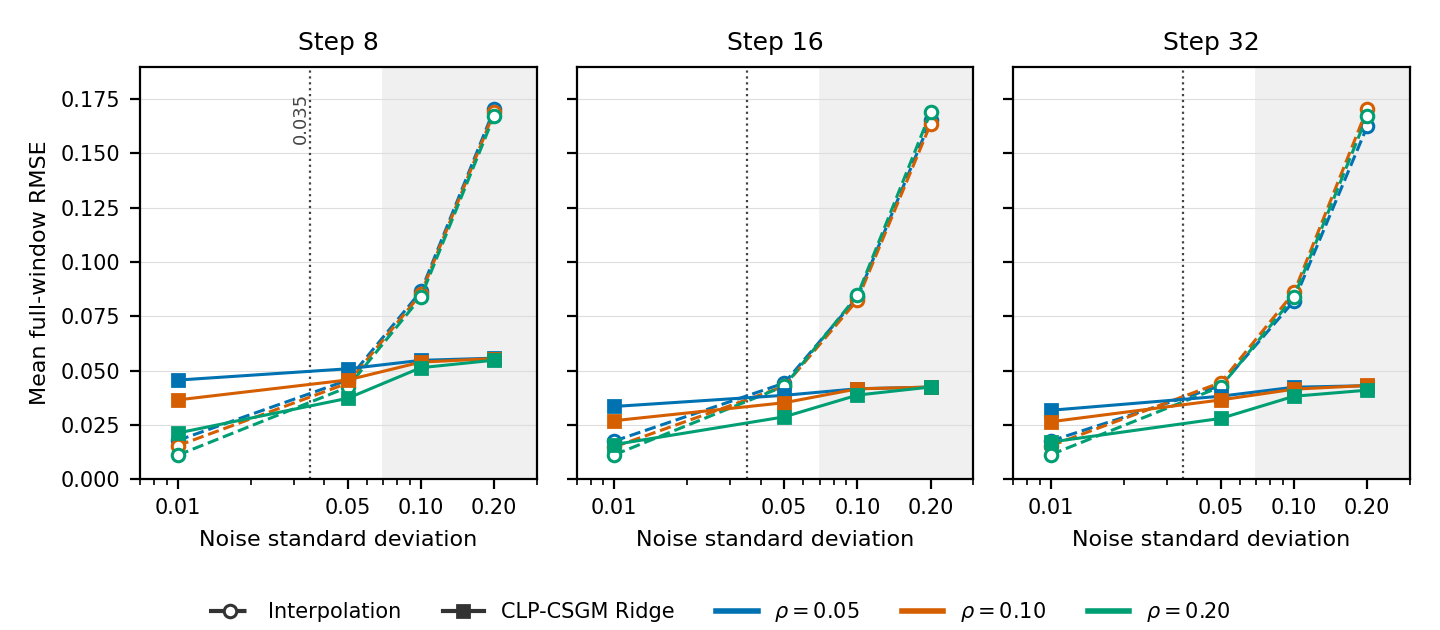
\includegraphics[width=\linewidth]{crosswell_vc_rmse_vs_noise.png}
    \caption{Mean full-window RMSE of depth interpolation and CLP-CSGM Ridge.
    The horizontal axis is logarithmic. Each panel is one step and each
    measurement fraction is a separate curve. Open circles are interpolation
    and squares are CLP-CSGM Ridge. Values are means over seeds $\{7,23,41\}$.
    The dotted line is the held-out $V_c$ standard deviation $0.035$, on the
    same scale as the noise. Noise $0.05$ is about $1.43$ times that
    deviation. The shaded region marks $0.10$ and $0.20$, about $2.86$ and
    $5.71$ times that deviation. These noise levels were used for
    sensitivity analysis and were not calibrated to field measurement
    uncertainties.
    The decoder and the dense-log map are fit once per step and seed. The
    penalty weight is selected on validation for each measurement fraction
    and each noise level. The points at noise $0.01$ belong to this refit.
    Cell means and seed-level win counts are reported in
    Table~\ref{tab:crosswell_noise_sweep}.}
    \label{fig:crosswell_rmse_vs_noise}
\end{figure}

Taken with the ten-seed panel, the two checks separate the randomness behind
the three-seed intervals: more seeds, each with its own coordinate draw, and
more coordinate draws at fixed model seeds. Both leave the submitted
three-seed tables unchanged. Overlapping windows are not counted as extra
independent samples.

\begin{table}[!htbp]
    \centering
    \caption{Paired seed-level
    $\Delta\mathrm{RMSE}=\mathrm{RMSE}_{\mathrm{AE}}-\mathrm{RMSE}_{\mathrm{CLP}}$
    on the cross-well $V_c$ grid ($n=3$ seeds). SE is the seed-level standard
    error; the $95\%$ half-width uses Student-$t$ with $\mathrm{df}=2$. Positive
    mean $\Delta\mathrm{RMSE}$ favors CLP-CSGM Ridge. Wins count seeds with
    strictly lower RMSE for each method.}
    \label{tab:paired_delta_crosswell}
    \small
    \adjustbox{max width=\linewidth}{
        \begin{tabular}{rrrrrrr}
\toprule
step & $\rho$ & mean $\Delta$RMSE & SE & $t_{2}$ 95\% half-width & CLP wins & AE wins \\
\midrule
8 & 0.05 & -0.00916 & 0.00350 & 0.01507 & 0 & 3 \\
8 & 0.10 & -0.00451 & 0.00231 & 0.00992 & 1 & 2 \\
8 & 0.20 & 0.00334 & 0.00200 & 0.00860 & 2 & 1 \\
16 & 0.05 & 0.00368 & 0.00123 & 0.00531 & 3 & 0 \\
16 & 0.10 & 0.00730 & 0.00187 & 0.00803 & 3 & 0 \\
16 & 0.20 & 0.01443 & 0.00362 & 0.01556 & 3 & 0 \\
32 & 0.05 & 0.00684 & 0.00120 & 0.00515 & 3 & 0 \\
32 & 0.10 & 0.01254 & 0.00216 & 0.00930 & 3 & 0 \\
32 & 0.20 & 0.02254 & 0.00202 & 0.00869 & 3 & 0 \\
\bottomrule
\end{tabular}

    }
\end{table}

Figure~\ref{fig:crosswell_all_methods} places the pairwise result within the full
benchmark. The mean RMSE of direct MLP and PCA increases sharply as training
support decreases, whereas AE has the lowest unweighted mean RMSE among the
direct baselines. Table~\ref{tab:crosswell_clp_vs_ae} therefore focuses on the
most competitive direct comparator in this grid.

\begin{figure}[!htbp]
    \centering
    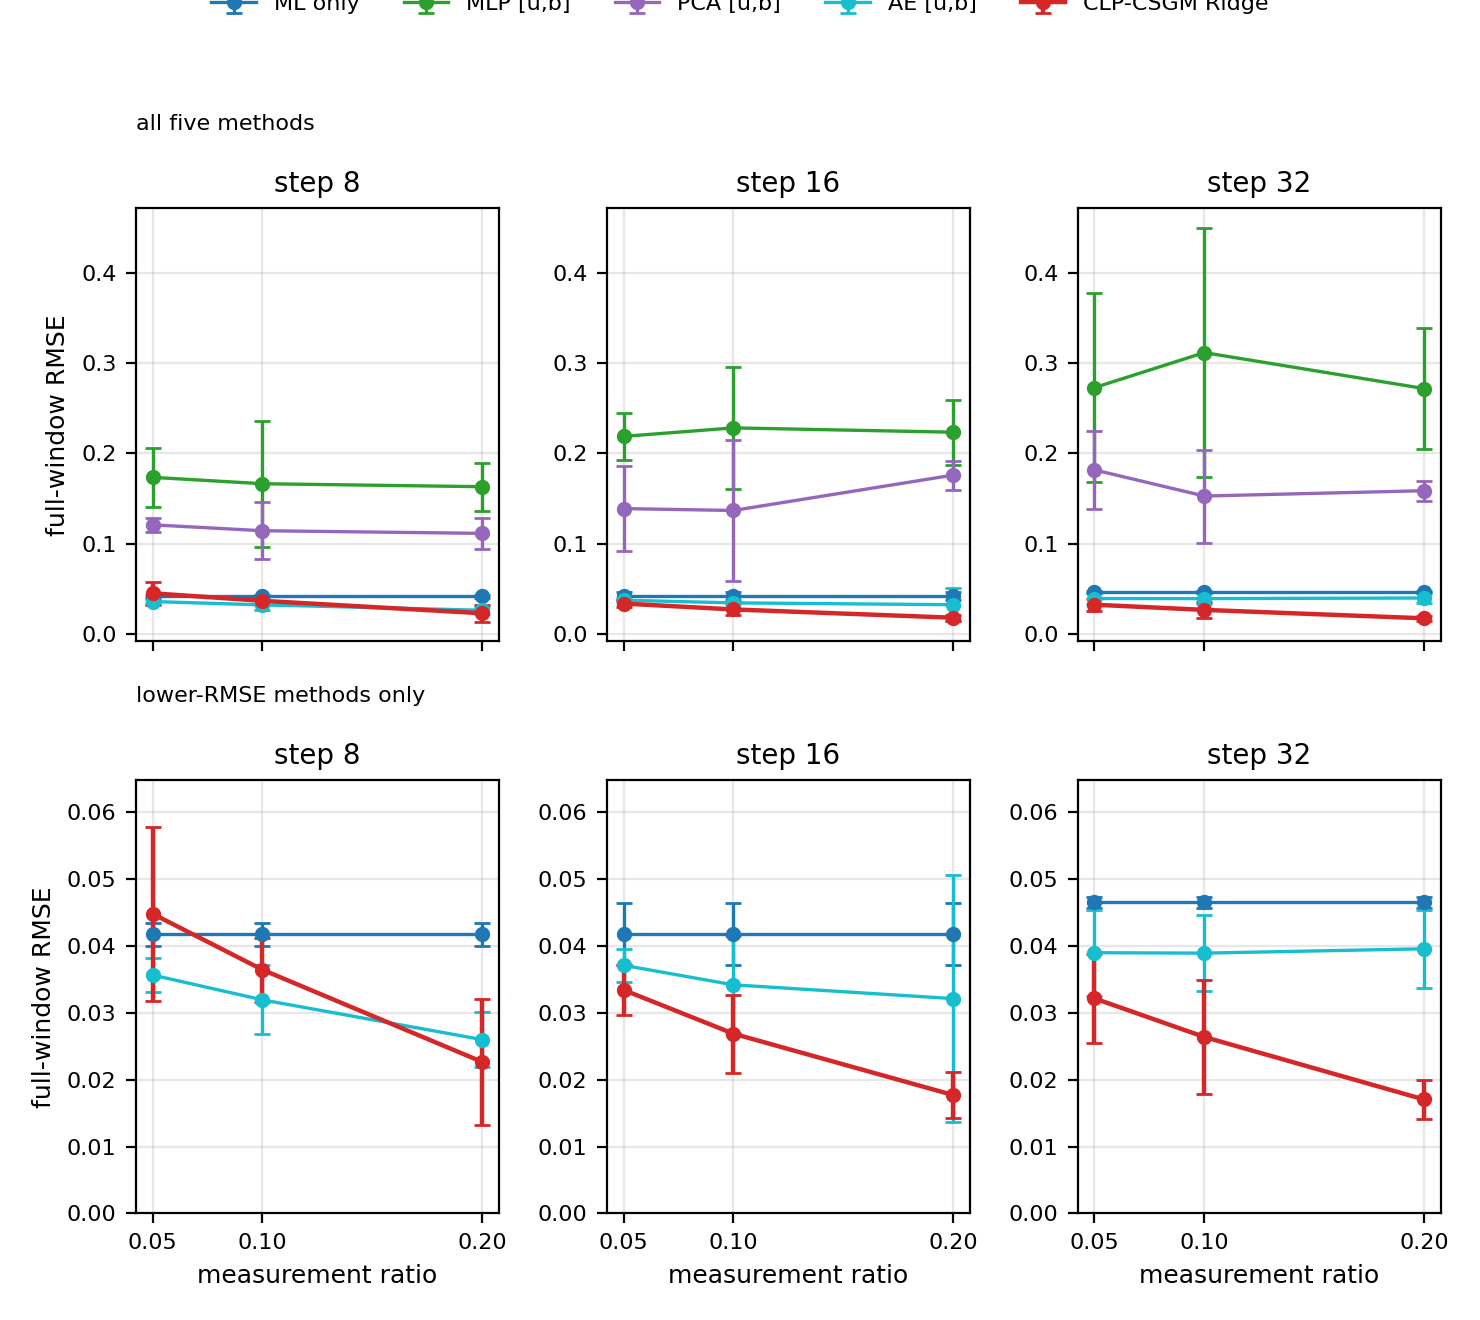
\includegraphics[width=\linewidth]{results_crosswell_rmse_vs_rho.png}
    \caption{Cross-well $V_c$ RMSE for the main methods. CLP-CSGM Ridge has the
    lowest mean RMSE in the medium-to-severe low-data cells, while the mean RMSE
    of direct MLP and PCA increases as training windows become scarce. Error
    bars are Student-$t$ $95\%$ half-widths across seeds ($\mathrm{df}=2$).}
    \label{fig:crosswell_all_methods}
\end{figure}

Figure~\ref{fig:crosswell_depth_profile} shows one held-out F03-4 profile
for step $16$, seed $7$, and $\rho=0.20$. In this displayed example,
CLP-CSGM Ridge follows the broad variations of the processed reference more
closely than AE $[\boldsymbol{u},\boldsymbol{b}]$. Direct MLP and PCA
predictions exhibit larger oscillations. Their panels use wider horizontal
scales than the reference, so that comparison is qualitative. The individual
window in Fig.~\ref{fig:sparse_recon_crosswell} is a different configuration:
step $16$, seed $7$, $\rho=0.10$, and window index 0. There, CLP-CSGM Ridge
is closer to the reference, the autoencoder prediction is positively offset,
and local deviations remain. These examples illustrate differences in
reconstruction behavior within the displayed configurations. They do not
establish a uniform advantage across the benchmark, and they are not a
statistical-significance claim. The profile is consistent with the aggregate
RMSE for this cell. Uniform window-level comparisons remain based on the
aggregate metrics.

\begin{figure}[!htbp]
    \centering
    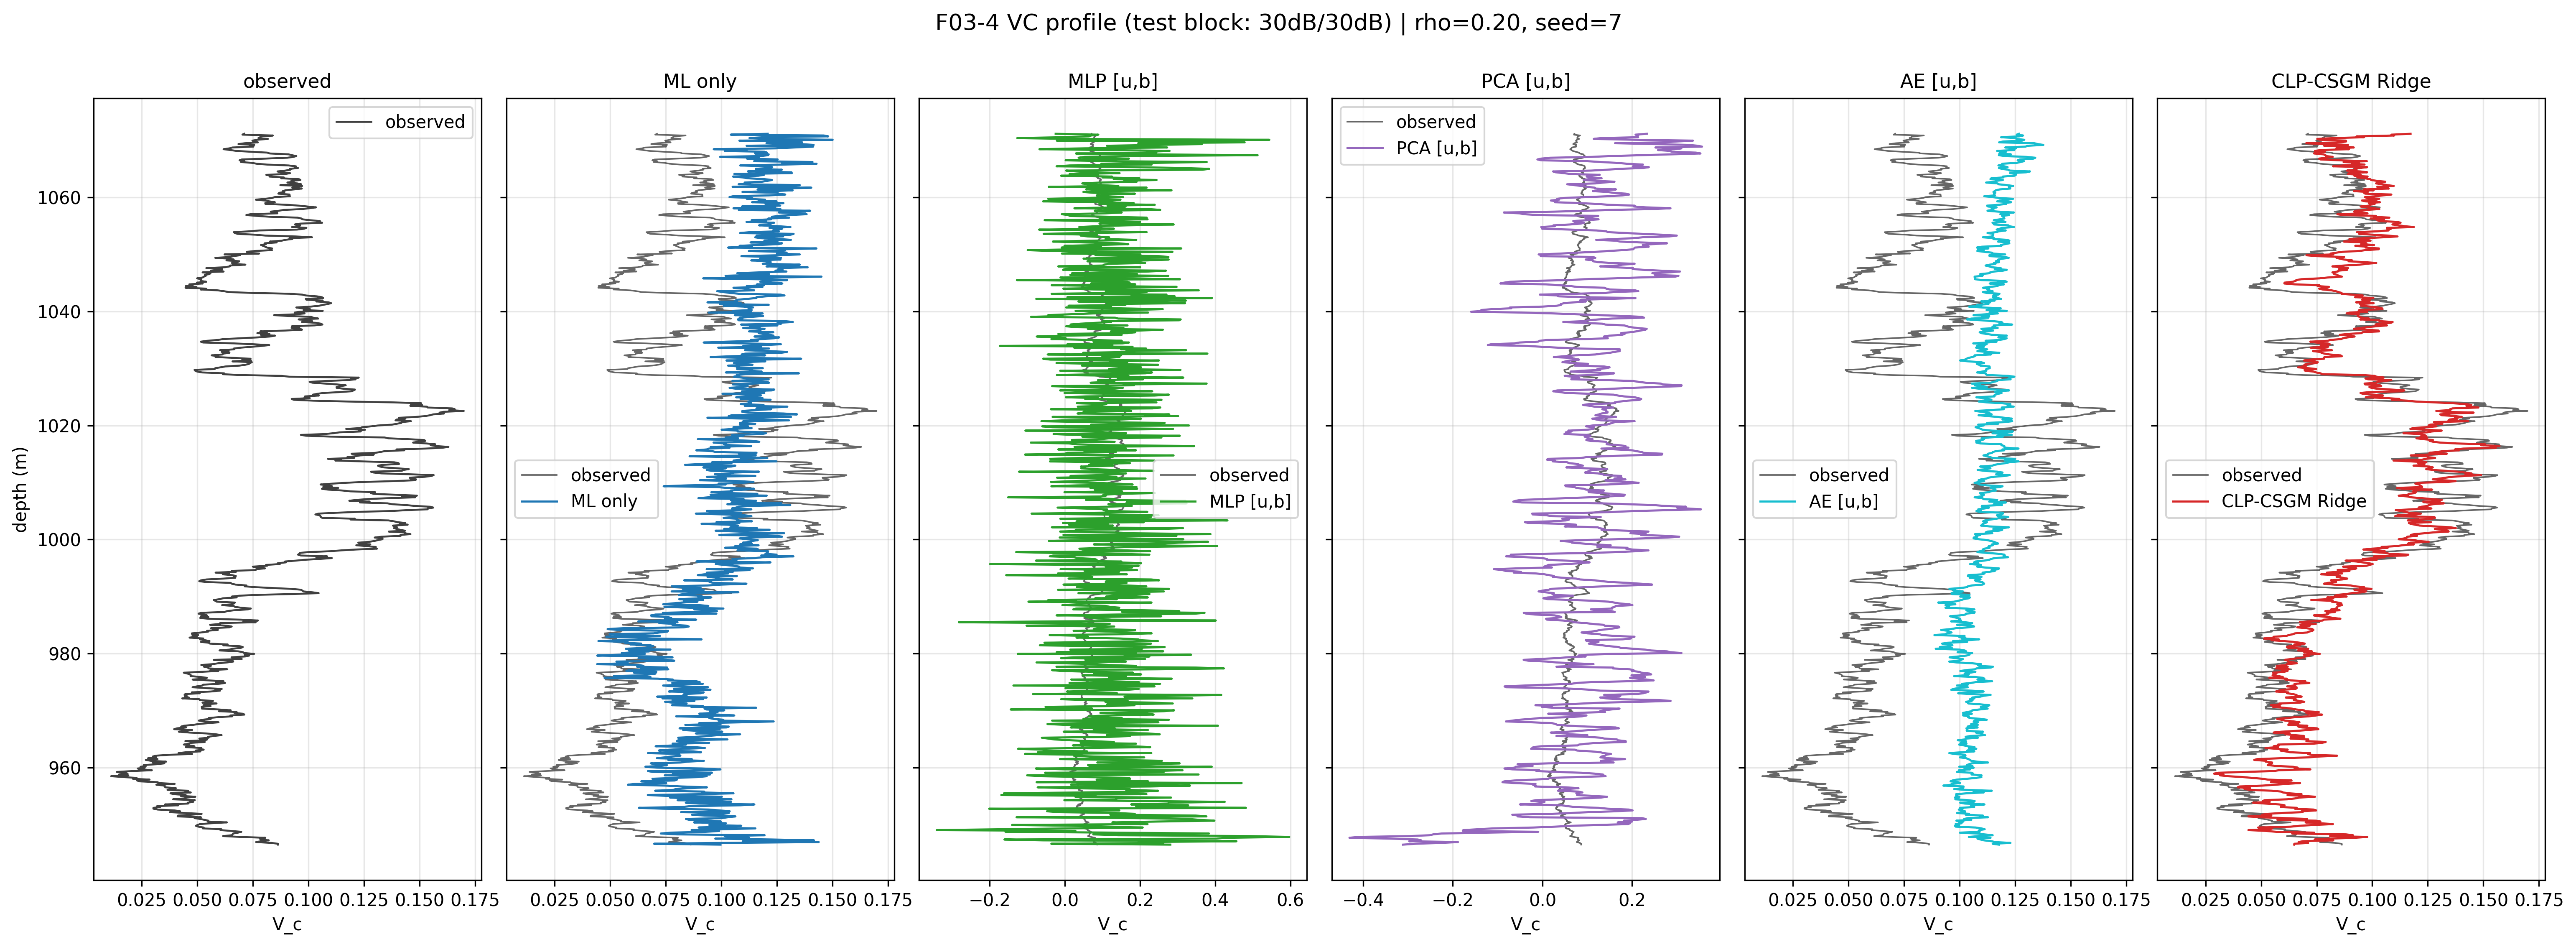
\includegraphics[width=\linewidth]{10_depth_profile_crosswell_vc.png}
    \caption{Held-out F03-4 $V_c$ reconstruction at step $16$, seed $7$, and
    $\rho=0.20$. The target is the processed Larionov-derived curve, and the
    sparse observations are coordinate subsamples of that curve. The MLP and
    PCA panels use wider horizontal scales than the reference panel.}
    \label{fig:crosswell_depth_profile}
\end{figure}

The paired step-$16$ checks in
Appendix~\ref{app:crosswell_gr_embargo}
(Table~\ref{tab:crosswell_gr_embargo_robustness}) show that including gamma ray
reduces absolute error and that the embargo changes training support, but
neither modification reverses the ordering of CLP-CSGM Ridge against AE
$[\boldsymbol{u},\boldsymbol{b}]$ and measurement-only CSGM at the tested
ratios.

\subsection{Single-well F03 GR-only results}
\label{subsec:f03_gr_only_results}

The F03-4 benchmark uses gamma ray as the only dense log. Table~\ref{tab:f03_results} shows that CLP-CSGM Ridge
achieves mean RMSE $0.01390$ across the tested grid, compared with $0.01434$
for AE $[\boldsymbol{u},\boldsymbol{b}]$. CLP-CSGM Ridge has lower mean RMSE at
$\rho\in\{0.20,0.30\}$, the methods are nearly tied at $\rho=0.50$, and AE has
lower mean RMSE at $\rho\in\{0.40,0.60\}$. In this benchmark, the largest
advantage of explicit latent refinement occurs at the sparsest ratios. Direct
AE fusion becomes competitive as more entries of $\boldsymbol{b}$ are
available.

\begin{table}[!htbp]
    \centering
    \caption{Single-well F03-4 GR-only porosity benchmark: mean RMSE by
    measurement ratio $\rho$. The prior-only and measurement-only rows are
    structural reference variants.}
    \label{tab:f03_results}
    \small
    \adjustbox{max width=\linewidth}{
        \begin{tabular}{lrrrrr}
\toprule
method & $\rho=0.20$ & $\rho=0.30$ & $\rho=0.40$ & $\rho=0.50$ & $\rho=0.60$ \\
\midrule
CLP-CSGM Ridge & 0.01596 & 0.01475 & 0.01377 & 0.01281 & 0.01220 \\
AE [u,b] & 0.01850 & 0.01554 & 0.01304 & 0.01286 & 0.01178 \\
Prior-only Ridge & 0.01958 & 0.01958 & 0.01958 & 0.01958 & 0.01958 \\
Measurement-only CSGM & 0.02519 & 0.02285 & 0.02033 & 0.01622 & 0.01494 \\
ML only & 0.02359 & 0.02359 & 0.02359 & 0.02359 & 0.02359 \\
PCA [u,b] & 0.02149 & 0.02187 & 0.02261 & 0.02409 & 0.02426 \\
MLP [u,b] & 0.03022 & 0.02997 & 0.03712 & 0.04199 & 0.04627 \\
\bottomrule
\end{tabular}

    }
\end{table}

Figure~\ref{fig:f03_gr_only_rmse} displays the complete comparison with
seed-level Student-$t$ $95\%$ half-widths ($\mathrm{df}=2$).
Table~\ref{tab:paired_delta_f03} reports the paired
$\Delta\mathrm{RMSE}=\mathrm{RMSE}_{\mathrm{AE}}-\mathrm{RMSE}_{\mathrm{CLP}}$
on the same three seeds: the mean gap is positive at $\rho=0.20$ and
$\rho=0.30$ (CLP wins all seeds), near zero at $\rho=0.50$, and negative at
$\rho\in\{0.40,0.60\}$ (AE wins all seeds). With $n=3$, several paired
intervals include zero. The F03 ordering therefore changes with how many
depths are measured, and the three-seed intervals are not a large-sample
significance claim. RMSE variability, MAE, and relative
$\ell_2$ error are reported in
Appendix~\ref{app:f03_full_table}
(Table~\ref{tab:f03_results_full}) and
Appendix~\ref{app:f03_metric_views}
(Figs.~\ref{fig:f03_mae}--\ref{fig:f03_rell2}); these metrics retain the same
regime-dependent interpretation.

\begin{table}[!htbp]
    \centering
    \caption{Paired seed-level
    $\Delta\mathrm{RMSE}=\mathrm{RMSE}_{\mathrm{AE}}-\mathrm{RMSE}_{\mathrm{CLP}}$
    on the F03-4 GR-only porosity benchmark ($n=3$ seeds). SE is the seed-level
    standard error; the $95\%$ half-width uses Student-$t$ with
    $\mathrm{df}=2$. Positive mean $\Delta\mathrm{RMSE}$ favors CLP-CSGM
    Ridge.}
    \label{tab:paired_delta_f03}
    \small
    \adjustbox{max width=\linewidth}{
        \begin{tabular}{rrrrrr}
\toprule
$\rho$ & mean $\Delta$RMSE & SE & $t_{2}$ 95\% half-width & CLP wins & AE wins \\
\midrule
0.20 & 0.00254 & 0.00042 & 0.00180 & 3 & 0 \\
0.30 & 0.00079 & 0.00032 & 0.00139 & 3 & 0 \\
0.40 & -0.00073 & 0.00035 & 0.00151 & 0 & 3 \\
0.50 & 0.00006 & 0.00033 & 0.00144 & 2 & 1 \\
0.60 & -0.00041 & 0.00024 & 0.00103 & 0 & 3 \\
\bottomrule
\end{tabular}

    }
\end{table}

\begin{figure}[!htbp]
    \centering
    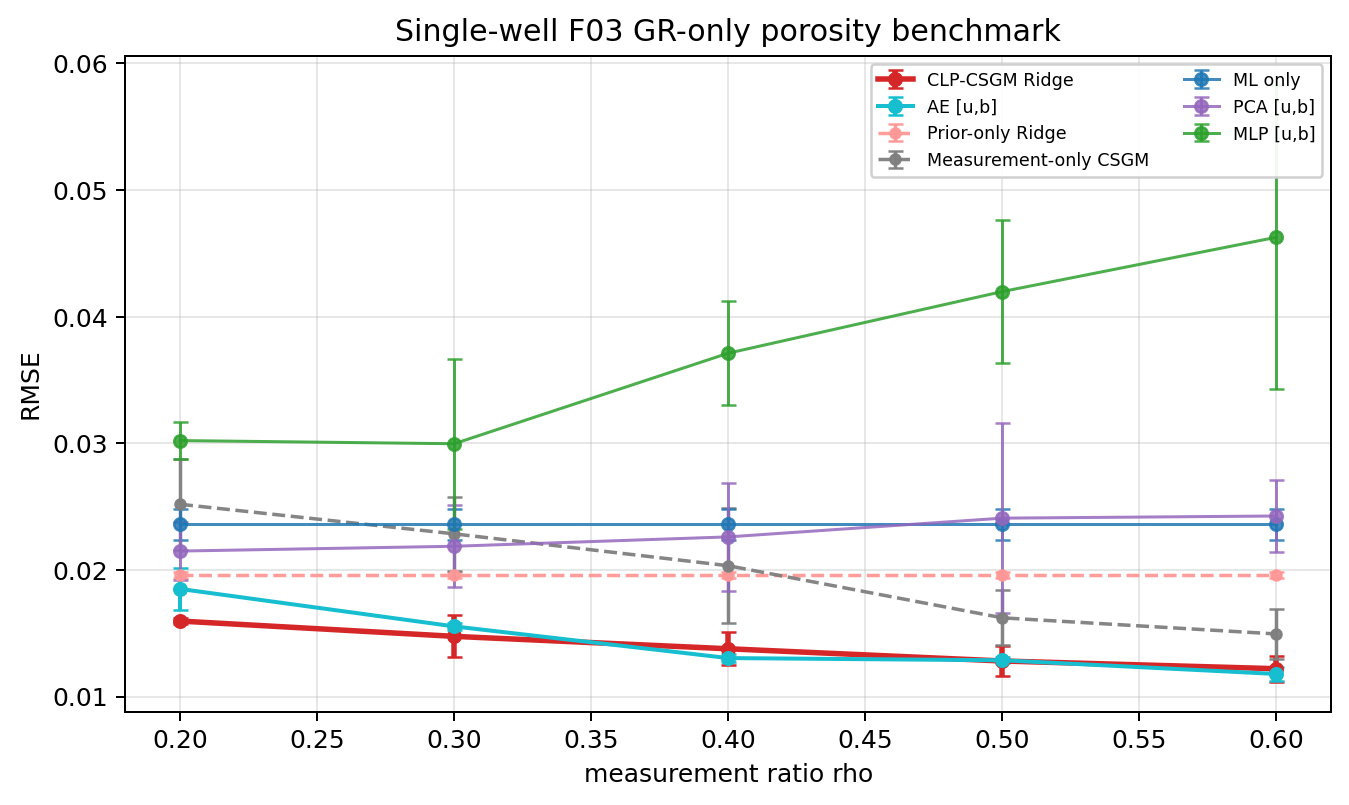
\includegraphics[width=0.72\linewidth]
    {results_f03_gr_only_rmse_vs_rho.png}
    \caption{F03-4 GR-only porosity RMSE by measurement ratio. CLP-CSGM Ridge
    has the lowest mean RMSE at the sparsest ratios, while AE
    $[\boldsymbol{u},\boldsymbol{b}]$ becomes competitive as more target
    observations are available. Error bars are Student-$t$ $95\%$ half-widths
    across seeds ($\mathrm{df}=2$).}
    \label{fig:f03_gr_only_rmse}
\end{figure}

The stress tests in Appendix~\ref{app:f03_stress}
(Table~\ref{tab:f03_stress}) extend the sparse grid to
$\rho\in\{0.05,0.10,0.20\}$. CLP-CSGM Ridge retains lower mean RMSE than AE
under increased noise and a smaller training pool, while the ordering becomes
less stable with a coarse sliding step and fewer test windows.

Figure~\ref{fig:f03_depth} shows the depth-profile reconstruction at
$\rho=0.20$, the main-grid ratio at which CLP-CSGM Ridge has its largest mean
RMSE advantage over the direct AE baseline.

\begin{figure}[!htbp]
    \centering
    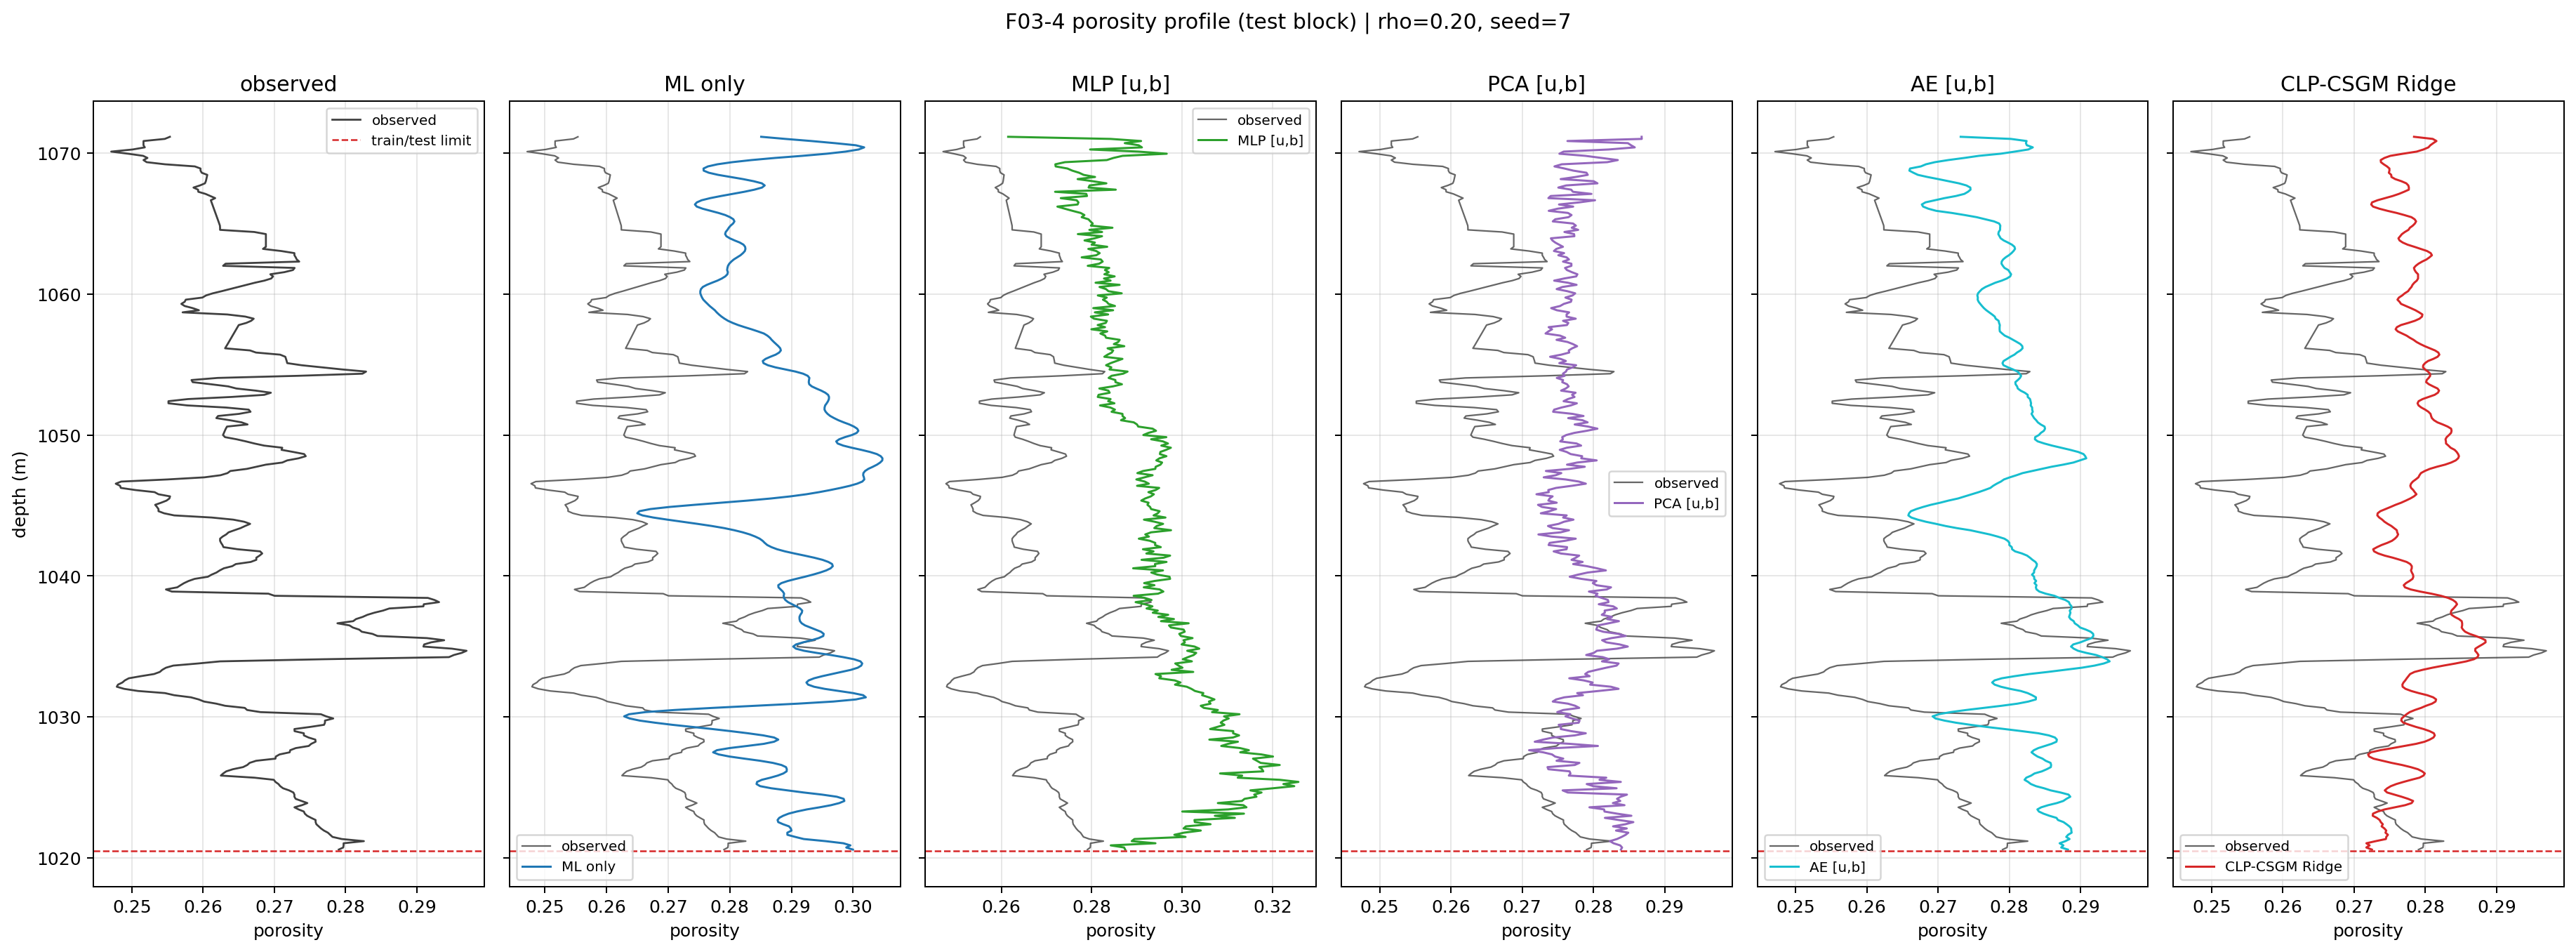
\includegraphics[width=0.90\linewidth]
    {10_depth_profile_porosity.png}
    \caption{F03-4 depth-profile reconstruction at $\rho=0.20$. The target is
    the processed density-derived porosity curve, and the sparse observations
    are coordinate subsamples of that curve. In this displayed profile,
    CLP-CSGM Ridge follows parts of the broad trend and smooths local
    variations. The panels do not share one horizontal scale.}
    \label{fig:f03_depth}
\end{figure}

The porosity example is more mixed than the clay-volume profile. In this
displayed profile, CLP-CSGM Ridge follows parts of the broad trend and smooths
local variations. Because the profile combines predictions from overlapping
windows, the view is qualitative. Pointwise recovery and validation against
independent core-porosity measurements fall outside this visualization. The
displayed window in Fig.~\ref{fig:sparse_recon_f03} uses the corresponding
configuration seed $7$, $\rho=0.20$, and window index 0. There, both
CLP-CSGM Ridge and AE $[\boldsymbol{u},\boldsymbol{b}]$ miss the central
depression of the reference. The pooled parity plot in
Fig.~\ref{fig:f03_parity} prints a correlation of $0.4632$ for CLP-CSGM Ridge
and $0.3720$ for the autoencoder. Those values describe the points drawn on
that figure. They do not establish statistical significance, and
overlapping-window predictions are not independent observations. The method
uses $m=13$ observations per length-$64$ window and achieves a mean RMSE of
approximately $0.016$ at $\rho=0.20$. This profile is consistent with the
lower mean RMSE in Table~\ref{tab:f03_results} at that ratio. The profile is
illustrative. The aggregate results still place the benefit of explicit latent
refinement at the sparse end of this weak-context grid.

The limited-sample Lapa permeability case in
Appendix~\ref{app:lapa_case} provides supplementary evidence. The prior-guided
CLP-CSGM variants have lower mean RMSE than the direct baselines that use
$[\boldsymbol{u},\boldsymbol{b}]$ across the tested grid. Their comparison with
measurement-only CSGM is ratio-dependent.

Appendix~\ref{app:phi_lab_861} scores laboratory porosity on held-out
coordinates of one cored interval. CLP-CSGM is not superior on the mean: the
direct AE has the lower RMSE at $\rho=0.25$ and $\rho=0.50$ ($0.0537$ and
$0.0523$, against $0.0602$ and $0.0580$ for CLP-CSGM Ridge). Laboratory
measurements still correct the log-only anchor, which CLP-CSGM Ridge beats in
every split. That correction is enough on the two shallower blocks, where the
test logs remain close to the support that fits the anchor and CLP-CSGM Ridge
has the lower block-mean RMSE. It does not close the gap on the deepest block,
where the logs shift and the decoded prediction $G(\boldsymbol{z}_0)$ differs substantially from the target windows. The
block RMSE, the log summaries, and the split counts are in
Appendix~\ref{app:phi_lab_861}.

\subsection{Ablation analysis}
\label{subsec:ablation_analysis}

The structural ablations drop one term at a time.
Prior-only returns the decoded prediction of the conditional prior,
$G(h(\boldsymbol{u}))$, with no latent search. Measurement-only
sets $\lambda=0$ and searches the decoder range using only the sparse
measurements \citep{bora2017compressed}. The comparison shows what each
term contributes
(Remark~\ref{rem:csgm_relation}).

In the cross-well benchmark, CLP-CSGM Ridge has lower mean RMSE than prior-only
in all nine cells, with reductions from $20.5\%$ to $60.6\%$
(Table~\ref{tab:ablation_crosswell}). It also has lower mean RMSE than
measurement-only CSGM in seven cells. The exceptions are step $8$ with
$\rho\in\{0.05,0.10\}$, where measurement-only CSGM has lower mean RMSE and the
Ridge code $\boldsymbol{z}_0$ is not beneficial. At steps $16$ and $32$, the full model has
lower mean RMSE than both ablations at every tested ratio.

\begin{table}[t]
    \centering
    \caption{Cross-well $V_c$ ablation results. Gains are relative RMSE
    reductions of CLP-CSGM Ridge with respect to the corresponding structural
    ablation; negative gain indicates that measurement-only CSGM has lower mean
    RMSE.}
    \label{tab:ablation_crosswell}
    \small
    \adjustbox{max width=\linewidth}{
        \begin{tabular}{rrrrrrrr}
\toprule
Step & $\rho$ & CLP-CSGM & Prior-only & Meas.-only & AE $[u,b]$ & Gain vs prior (\%) & Gain vs meas. (\%) \\
\midrule
8 & 0.0500 & 0.0448 & 0.0564 & 0.0368 & 0.0357 & 20.4913 & -21.7274 \\
8 & 0.1000 & 0.0365 & 0.0564 & 0.0297 & 0.0320 & 35.3433 & -22.7163 \\
8 & 0.2000 & 0.0227 & 0.0564 & 0.0251 & 0.0260 & 59.8016 & 9.5581 \\
16 & 0.0500 & 0.0334 & 0.0426 & 0.0362 & 0.0371 & 21.5310 & 7.6727 \\
16 & 0.1000 & 0.0269 & 0.0426 & 0.0295 & 0.0342 & 36.8933 & 8.9585 \\
16 & 0.2000 & 0.0177 & 0.0426 & 0.0213 & 0.0321 & 58.4391 & 16.7449 \\
32 & 0.0500 & 0.0322 & 0.0432 & 0.0341 & 0.0390 & 25.5774 & 5.6452 \\
32 & 0.1000 & 0.0264 & 0.0432 & 0.0271 & 0.0389 & 38.9248 & 2.4363 \\
32 & 0.2000 & 0.0170 & 0.0432 & 0.0219 & 0.0396 & 60.5584 & 22.0073 \\
\bottomrule
\end{tabular}

    }
\end{table}

In the F03-4 GR-only benchmark, CLP-CSGM Ridge has lower mean RMSE than both
ablations at every tested ratio (Table~\ref{tab:ablation_f03}). Its reduction
relative to prior-only
increases from approximately $18.5\%$ at $\rho=0.20$ to $37.7\%$ at
$\rho=0.60$, while its largest gains over measurement-only occur at the
sparsest ratios. Both terms contribute. The cross-well exceptions show that
the conditional code $\boldsymbol{z}_0$ is not helpful in every cell.

\begin{table}[t]
    \centering
    \caption{Single-well F03-4 GR-only ablation results. Gains are relative
    RMSE reductions of CLP-CSGM Ridge with respect to the corresponding
    structural ablation.}
    \label{tab:ablation_f03}
    \small
    \adjustbox{max width=\linewidth}{
        \begin{tabular}{rrrrrrr}
\toprule
$\rho$ & CLP-CSGM & Prior-only & Meas.-only & AE $[u,b]$ & Gain vs prior (\%) & Gain vs meas. (\%) \\
\midrule
0.2000 & 0.0160 & 0.0196 & 0.0252 & 0.0185 & 18.4646 & 36.6254 \\
0.3000 & 0.0148 & 0.0196 & 0.0228 & 0.0155 & 24.6433 & 35.4375 \\
0.4000 & 0.0138 & 0.0196 & 0.0203 & 0.0130 & 29.6514 & 32.2641 \\
0.5000 & 0.0128 & 0.0196 & 0.0162 & 0.0129 & 34.5823 & 21.0300 \\
0.6000 & 0.0122 & 0.0196 & 0.0149 & 0.0118 & 37.6999 & 18.3817 \\
\bottomrule
\end{tabular}

    }
\end{table}

\subsection{Latent-prior model sensitivity}
\label{subsec:latent_prior_sensitivity}

Tables~\ref{tab:prior_class_crosswell} and~\ref{tab:prior_class_f03} compare
Ridge and MLP implementations of $h$ while keeping the remaining pipeline
fixed. This sensitivity analysis is limited to these two prior classes. Signed
Ridge gain is defined as
$100(\mathrm{RMSE}_{\mathrm{MLP}}-\mathrm{RMSE}_{\mathrm{Ridge}})
 /\mathrm{RMSE}_{\mathrm{MLP}}$; positive values favor Ridge.

In the cross-well benchmark, MLP has lower mean RMSE in all nine cells. The
relative difference is largest at sparse measurement ratios and decreases as
$\rho$ increases; at step $16$, for example, signed Ridge gain changes from
approximately $-82\%$ at
$\rho=0.05$ to $-26\%$ at $\rho=0.20$. Ridge remains the headline comparator
for the reason in Section~\ref{sec:discussion}: a fixed linear reference, not
a claim that it dominates MLP on this grid.

\begin{table}[t]
    \centering
    \caption{Cross-well $V_c$ latent-prior sensitivity. Positive signed Ridge
    gain favors Ridge, whereas negative values favor MLP.}
    \label{tab:prior_class_crosswell}
    \small
    \adjustbox{max width=\linewidth}{
        \begin{tabular}{rrrrr}
\toprule
Step & $\rho$ & CLP-CSGM MLP & CLP-CSGM Ridge & Ridge gain (\%) \\
\midrule
8 & 0.0500 & 0.0183 & 0.0448 & -144.8574 \\
8 & 0.1000 & 0.0171 & 0.0365 & -112.7948 \\
8 & 0.2000 & 0.0138 & 0.0227 & -64.3792 \\
16 & 0.0500 & 0.0183 & 0.0334 & -82.4082 \\
16 & 0.1000 & 0.0175 & 0.0269 & -53.3581 \\
16 & 0.2000 & 0.0141 & 0.0177 & -25.8526 \\
32 & 0.0500 & 0.0221 & 0.0322 & -45.4853 \\
32 & 0.1000 & 0.0212 & 0.0264 & -24.5143 \\
32 & 0.2000 & 0.0158 & 0.0170 & -7.7698 \\
\bottomrule
\end{tabular}

    }
\end{table}

In the F03-4 GR-only benchmark, Ridge has lower mean RMSE at every tested ratio,
but the relative difference decreases from approximately $14.3\%$ at
$\rho=0.20$ to $1.7\%$ at $\rho=0.60$.

\begin{table}[t]
    \centering
    \caption{Single-well F03-4 GR-only latent-prior sensitivity. Signed Ridge
    gain follows the definition used in
    Table~\ref{tab:prior_class_crosswell}.}
    \label{tab:prior_class_f03}
    \small
    \adjustbox{max width=\linewidth}{
        \begin{tabular}{rrrr}
\toprule
$\rho$ & CLP-CSGM MLP & CLP-CSGM Ridge & Ridge gain (\%) \\
\midrule
0.2000 & 0.0186 & 0.0160 & 14.2682 \\
0.3000 & 0.0167 & 0.0148 & 11.4868 \\
0.4000 & 0.0152 & 0.0138 & 9.2929 \\
0.5000 & 0.0132 & 0.0128 & 2.6767 \\
0.6000 & 0.0124 & 0.0122 & 1.6615 \\
\bottomrule
\end{tabular}

    }
\end{table}

Which map is better depends on the dataset and on how many depths are
measured, and the difference shrinks as more target values enter
$\boldsymbol{b}$. Ridge stays the reported reference because it is a fixed
linear map, not because it wins every cell. The rankings support choosing
that map on validation data for the intended test, rather than after seeing
the held-out result.

\paragraph{Supplementary diagnostics.}
Appendix~\ref{app:validation_generalization_diagnostics} audits validation,
selected $\lambda$, and per-window errors;
Appendix~\ref{app:sparse_recon_examples} shows realized sparse-measurement
windows; Appendix~\ref{app:separability} assesses empirical decoder-range
separation; and Appendix~\ref{app:runtime} reports inference cost. These
analyses serve interpretive and reproducibility purposes and are separate from
the benchmark comparisons.
